\chapter{Materiais e Métodos}
\label{chap:mat}
asdfasdfsdf

%--------- NEW SECTION ----------------------
\section{Especificação dos componentes}
\label{sec:espc}
asjdflkdjsaf

\subsection{Estrutura analítica do protótipo}
\label{ssec:pbs}
asdkjfsdalkjf

\subsection{Lista de componentes}
\label{ssec:list}
asfkjdsahfkjs


%--------- NEW SECTION ----------------------
\section{Diagramas mecânicos}
\label{sec:diagm}
asdfsdaf

%--------- NEW SECTION ----------------------
\section{Modelo esquemático de alimentação e comunicação}
\label{sec:modesq}
asdfadsfsdfs

\subsection{Diagramas elétricos}
\label{sec:diage}
asdfsdaf

\subsection{Esquemas eletrônicos}
\label{ssec:esqe}
asdfsdaf

%--------- NEW SECTION ----------------------
\section{Especificação das funcionalidades}
\label{sec:espf}
asdfadsfsdfs

\subsection{Fluxo das informações}
\label{ssec:fluxo}
asdfsaf

\subsection{Motion Planning}
\label{ssec:func1}
\subsubsection{Definição da funcionalidade}
A funcionalidade de \textit{Motion Planning} é responsável por realizar o planejamento da trajetória do Robô, utilizando o software \textit{MoveIt!} que realiza o cálculo da cinemática inversa para encontrar a melhor forma de ultrapassar os obstáculos.
\subsubsection{Dependências}
O software moveit pode utilizar o modelo matemático da cinemática inversa do robô ou um arquivo do tipo URDF.
O nome URDF é uma sigla para \textit{Unified Robot Description Format}, esse arquivo é uma especificação em \verb|XML| utilizada para descrever robôs. Modelos em URDF apresentam uma simplicidade na descrição do robô, e para o caso do Robô \textit{Elir}, utilizar o modelo URDF possibilitará uma aproximação fiel ao modelo real do robô, assim para o cálculo da cinemática inversa será utilizado o seu modelo URDF e não o seu modelo matemático.

\subsubsection{Premissas Necessárias}
Para o correto funcionamento dessa funcionalidade as seguintes premissas são necessárias:
\begin{itemize}
	\item A configuração dos limites de giro das juntas do robô estarão compatíveis com os comandos enviados
	\item O modelo URDF do robô estará adequado com o modelo físico
	\item O pacote gerado pelo \textit{MoveIt! Setup Assistant} estará configurado adequadamente
\end{itemize}
\subsubsection{Descrição da Funcionalidade}
A movimentação do robô na linha acontecerá por movimentos de translação e transposição de obstáculos. A translação na linha será feita por controladores de torque nas rodas do robô, enquanto a transposição do obstáculos utilizará o moveit.
Por meio da ferramenta \textit{MoveIt! Setup Assistant}, se utiliza o modelo do robô para criar um pacote do ROS com os principais arquivos pelo moveit. 
A configuração correta do moveit possibilita que se utilizem as funções da sua biblioteca para o cálculo da trajetória, levando em consideração também obstáculos no caminho.

O moveit fornece uma \textit{user interface} que recebe o end-effector,a nomenclatura atribuída ao node feito em python que recebe o \textit{end-effector} é \verb|moveit_commander|. O  \textit{node} responsável por fazer a integração da user interface com os parâmetros recebidos pelo \textit{ROS Parameter Server} com o \textit{end-effector} para fazer os cálculos é denominado \verb|move_group|. O \textit{node} \verb|move_group| também pode receber parâmetros como leituras dos sensores do robô e nuvens de pontos.

\begin{figure}[h]
	\centering
	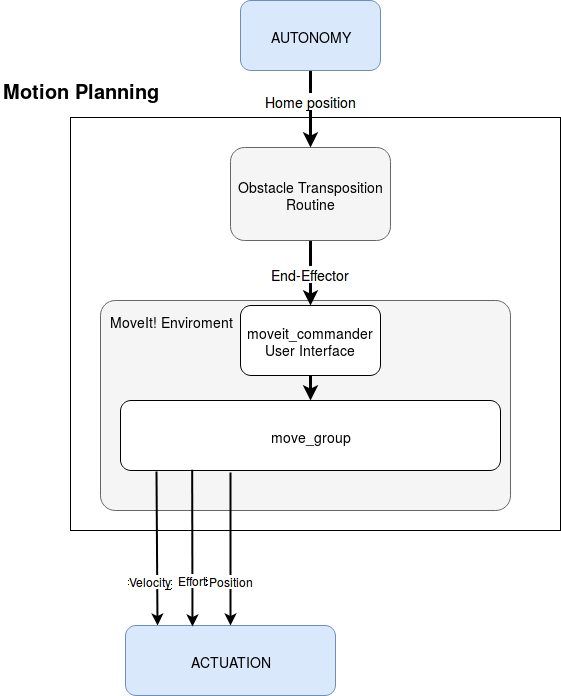
\includegraphics[width=0.6\textwidth]{motion_plan_func.png}
	\caption{Fluxograma de funcionamento da funcionalidade de Motion Planning}
	\label{fig:flux_motion}
	\source{Própria}
\end{figure}

\subsubsection{Saídas}
Por meio da compatibilização do \textit{MoveIt!} com o \textit{ROS}, a saída dessa funcionalidade são os comandos de velocidade, esforço e posição para cada junta do robô.

\subsection{Funcionalidade 2}
\label{ssec:func2}
asdfsaf

\subsection{Funcionalidade 3}
\label{ssec:func3}
asdfsaf

%--------- NEW SECTION ----------------------
\section{Interface do Usuário}
\label{sec:ui}
asdfadsfsdfs

%--------- NEW SECTION ----------------------
\section{Simulação do sistema}
\label{sec:sim}
asdfadsfsdfs


